\documentclass{ctexart}
\usepackage{graphicx}
\usepackage{caption}
\usepackage{float}
\usepackage{amsmath}
\usepackage{fancyhdr}
\usepackage{xunicode-addon}
\usepackage{booktabs}
\usepackage[a4paper,hmargin=1.25in,vmargin=1in]{geometry}
% !TeX program = xelatex
\title{\begin{figure}[H]
	\centering 
	\includegraphics[height=7cm,width=14cm]{E:/Pictures/中科大.jpg}
	\end{figure}\Huge\textbf{Lab 2}\\\huge{线性方程组求解}}
\date{}
\punctstyle{banjiao} 
\pagestyle{fancy}
	\fancyhead[C]{\LARGE\textbf{Lab 2}}
	\fancyhead[L]{}
	\fancyhead[R]{}
	\fancyfoot[C]{\thepage}
\begin{document}
	\maketitle
	\thispagestyle{empty}
	
	\[\makebox{\Large{姓名:\underline{\makebox[5cm]{高茂航}}}}\]
	
    \[\makebox{\Large{学号:\underline{\makebox[5cm]{PB22061161}}}}\]
	
	$$\makebox{\Large{日期:\underline{\makebox[5cm]{2024.3.28}}}}$$
	
	\clearpage

	\pagenumbering{arabic}

	\section{Algorithm Description}
	已知$y_0=0,y_{100}=1$,解线性方程组$\mathbf{A}\mathbf{y} = \mathbf{b}$,其中
\[\mathbf{A_{99\times99}}= \begin{bmatrix}
        -(2\epsilon + h) & \epsilon + h & 0 & \cdots & 0 \\
        \epsilon & -(2\epsilon + h) & \epsilon + h & \cdots & 0 \\
        0 & \epsilon & -(2\epsilon + h) & \cdots & 0 \\
        \vdots & \vdots & \ddots & \ddots & \vdots \\
        0 & 0 & \cdots&  \epsilon& -(2\epsilon + h) \\
        \end{bmatrix}\]

			\begin{align*}
			\mathbf{y} = \begin{bmatrix}
						y_1 \\
						y_2 \\
						y_3 \\
						\vdots \\
						y_{99} \\
						\end{bmatrix}
			\quad & \quad
			\mathbf{b}= \begin{bmatrix}
							ah^2 \\
							ah^2 \\
							\vdots \\
							ah^2 \\
							ah^2-\epsilon-h
							\end{bmatrix}
			\end{align*}
			设相对误差$\text{err} = \frac{1}{99}\displaystyle\sum_{i=1}^{99} |y_i - \text{Precise}_i|$。

\subsection{列主元消元法}
记录当前所处的位置A[col][col],在第col行到最后一行中找到绝对值最大的元素,将该元素所在的行与第col行交换,然后将第col行下的所有行的第col列元素变为0。重复这个过程,直到col=n-1,将矩阵化为上三角矩阵,再通过回代求解线性方程组。
\subsection{Gauss-Seidel迭代法}
		
$$\mathbf{X^{(k+1)}}=-(\mathbf{D}+\mathbf{L})^{-1}\mathbf{U}\mathbf{X^{(k)}}+(\mathbf{D}+\mathbf{L})^{-1}\mathbf{b}$$
    令            
	\begin{align*}
		\mathbf{S} &= -(\mathbf{D}+\mathbf{L})^{-1}\mathbf{U} \\
		&= \begin{bmatrix}
		0 & \frac{\epsilon + h}{2\epsilon + h} & 0 & \cdots & 0 \\
		0 & \frac{\epsilon(\epsilon + h)}{(2\epsilon + h)^2}  & \frac{\epsilon + h}{2\epsilon + h}& \cdots & 0 \\
		0 & \frac{\epsilon^2(\epsilon + h)}{(2\epsilon + h)^3} & \frac{\epsilon(\epsilon + h)}{(2\epsilon + h)^2} & \ddots & 0 \\
		\vdots & \vdots & \vdots & \ddots & \vdots \\
		0 & \frac{\epsilon^{n-1}(\epsilon + h)}{(2\epsilon + h)^n} &  \frac{\epsilon^{n-2}(\epsilon + h)}{(2\epsilon + h)^{n-1}} & \cdots & \frac{\epsilon(\epsilon + h)}{(2\epsilon + h)^2} \\
		\end{bmatrix}
		\end{align*}
	
	\begin{align*}
	\mathbf{Inv} &= (\mathbf{D}+\mathbf{L})^{-1} \\
	&= \begin{bmatrix}
	-\frac{1}{2\epsilon + h} & 0 & 0 & \cdots & 0 \\
	-\frac{\epsilon}{(2\epsilon + h)^2} & -\frac{1}{2\epsilon + h} & 0 & \cdots & 0 \\
	-\frac{\epsilon^2}{(2\epsilon + h)^3} & -\frac{\epsilon}{(2\epsilon + h)^2} & -\frac{1}{2\epsilon + h} & \cdots & 0 \\
	\vdots & \vdots & \vdots & \ddots & \vdots \\
	-\frac{\epsilon^{n-1}}{(2\epsilon + h)^n} & -\frac{\epsilon^{n-2}}{(2\epsilon + h)^{n-1}} & \cdots & -\frac{\epsilon}{(2\epsilon + h)^2} & -\frac{1}{2\epsilon + h} \\
	\end{bmatrix}
	\end{align*}
	在$\|\mathbf{X^{(k+1)}}-\mathbf{X^{(k)}}\|_{\infty}\leq10^{-6}$时结束迭代。
	
\section{Results}

\begin{figure}[H]
	\centering 
	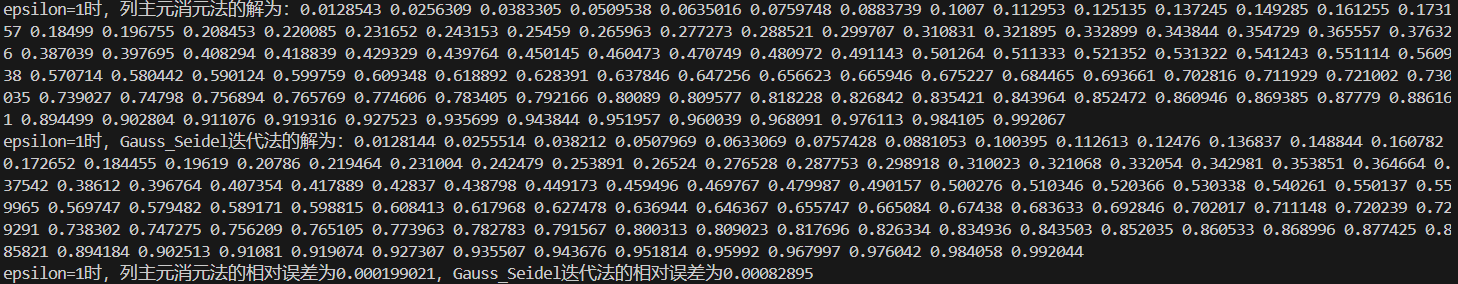
\includegraphics[height=3cm,width=14cm]{1.png}
	\end{figure}
	\begin{figure}[H]
		\centering 
		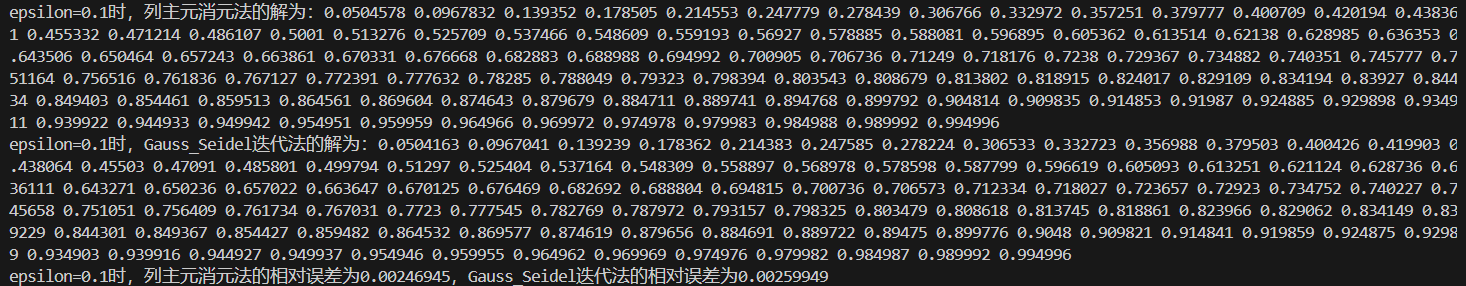
\includegraphics[height=3cm,width=14cm]{2.png}
		\end{figure}
		\begin{figure}[H]
			\centering 
			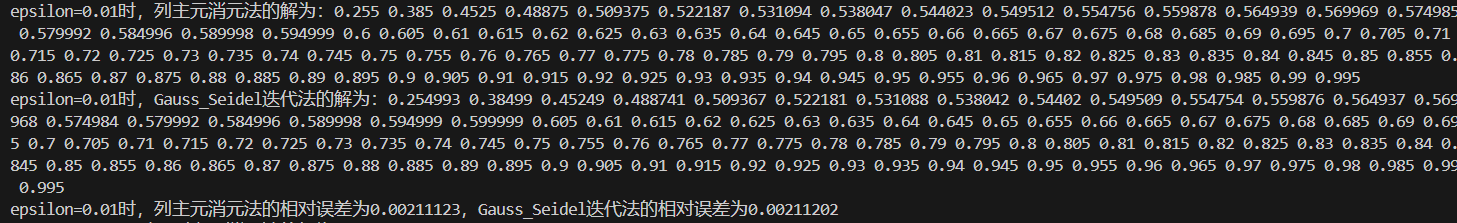
\includegraphics[height=2.5cm,width=14cm]{3.png}
			\end{figure}
			\begin{figure}[H]
				\centering 
				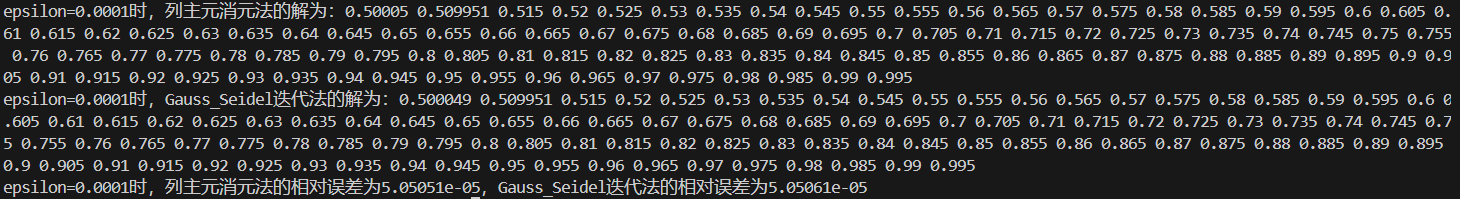
\includegraphics[height=2cm,width=14cm]{4.png}
				\end{figure}
	\section{Conclusion}
从结果可看出,列主元消元法和Gauss-Seidel迭代法的结果基本一致,且相对误差均在$10^{-4}$量级内,说明两种方法都能较好地解决线性方程组问题。
但列主元消元法的精度相对更高,且耗时更短。

本实验提高精度的主要措施:

1.使用long double类型;

2.提前计算好$\mathbf{S}$和$\mathbf{Inv}$的形式,再代入数值,以避免用代码求逆矩阵和进行矩阵乘法时产生的误差。


但由于本题矩阵阶数较大,而且矩阵元素的分子分母次数较高,同时消元、迭代等运算需要大量进行,因此在计算过程中误差会逐渐积累,导致最终结果的精度难以把握,只能控制在一定范围内。
\end{document}